\scanpage{65}
\[
\pi_1(X\times Y)\xrightarrow{\underline{\mathrm{surj}}}\pi_1(X)\times\pi_1(Y)
\]

\diagram{\begin{tikzcd}[ampersand replacement=\&,column sep=small]
X\arrow[d]\&[-1em]\supset Z\\
Y\&{}
\end{tikzcd}}

\[
\pi_1(Z)\unsure{\longrightarrow|-}\pi_1(X)\unsure{\longrightarrow|-}\pi_1(Y)
\]

\diagram{\begin{tikzcd}[ampersand replacement=\&,row sep=small]
X''\arrow[d,shift left=.6ex]\arrow[d,shift right=.6ex]\\
X'\arrow[d]\\
X\arrow[d]\\
\cdot
\end{tikzcd}}

\figure{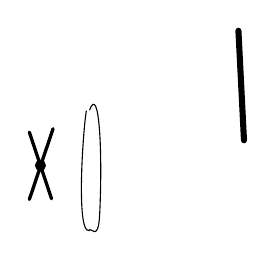
\begin{tikzpicture}[x=.47cm,y=.47cm,line cap=round]
\draw[very thick] (-.3,.9)--(.3,-.9) (-.3,-.92)--(.34,.99);
\fill (0,0) circle (.15);
\draw (1.33,1.50) .. controls (1.60,2.22) and (1.68,.26) .. (1.60,-1.33) .. controls (1.56,-2.11) and (1.36,-1.63) .. (1.31,-1.76) .. controls (.96,-1.82) and (1.15,.96) .. (1.24,1.47);
\draw[line width=2.2pt] (5.35,3.64)--(5.50,.68);
\end{tikzpicture}}

\diagram{\begin{tikzcd}[ampersand replacement=\&,column sep=small,row sep=0pt]
X\&\subset\&\widehat X\&\text{\unsure{normaux}}\\
\rotatebox{90}{$\subset$}\&{}\&\rotatebox{90}{$\subset$}\&{}\\
X_0\&\subset\&\deleted{\unsure{X}}\widehat X_0\&\text{pts singuliers}
\end{tikzcd}}

\figure{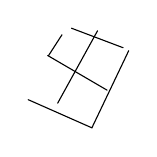
\begin{tikzpicture}[x=.55cm,y=.55cm,line cap=round]
\draw (-.77,.48)--(-.46,.96) (-.79,.48)--(.58,-.32) (-.24,1.11)--(.95,.66);
\draw (.36,1.05)--(-.56,-.62) (1.08,.59)--(.23,-1.19)--(-1.24,-.54);
\end{tikzpicture}}

\diagram{\begin{tikzcd}[ampersand replacement=\&,column sep=small,row sep=small]
Y'\arrow[r,dash]\arrow[d]\&X'\arrow[d]\\
Y\&[-.5em]{}\llap{$\subset\;$}X\arrow[d]\\
{}\&P^{r}
\end{tikzcd}}

\diagram{\begin{tikzcd}[ampersand replacement=\&,column sep=small,row sep=small]
X'\arrow[d]\&\subset\&\overline{X}'\arrow[d]\\
X\arrow[d]\&\subset\&\overline X\arrow[dll]\\
P^r\&{}\&{}
\end{tikzcd}}

\diagram{\begin{tikzcd}[ampersand replacement=\&,column sep=small,row sep=small]
Y\arrow[r]\arrow[d]\&X\arrow[d]\\
H\arrow[r]\&P^r\\[-.75em]
/K\&/k
\end{tikzcd}}

\[
\pi_1(Y)\longrightarrow\pi_1(X)
\]
$X$ normal

\[
\pi_1(Y')\xrightarrow{\mathrm{surj}??}\pi_1(X)
\]

\[
\pi_1(X)
\]

\figure{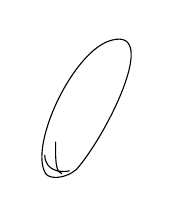
\begin{tikzpicture}[x=.60cm,y=.60cm,line cap=round]
\draw (.06,.06) .. controls (-.31,.65) and (.66,2.71) .. (1.47,2.89) .. controls (2.46,3.14) and (1.38,.92) .. (.71,.15) .. controls (.47,-.05) and (.15,-.06) .. (.06,.06);
\draw (.04,.45) .. controls (.05,.12) and (.37,.08) .. (.56,.12) (.27,.73) .. controls (.26,.20) and (.30,.10) .. (.40,.06);
\end{tikzpicture}}

\[
\deleted{\pi_1(Y)\to\pi_1(X)\leftarrow\pi_1(X-Y)}
\]
% archive sheet number: 64
